\documentclass[a4paper]{article}

\usepackage{times}
\usepackage{tikz}
\usepackage[margin=0cm]{geometry}
\usepackage{graphicx}
\usepackage{anyfontsize}
\usepackage{fancyhdr}
\usepackage{indentfirst}
\usepackage{amsmath}
\usepackage[spanish]{babel}
\usepackage[utf8]{inputenc}
\usepackage{titlesec}
\usepackage{booktabs}
\usepackage{multicol}

\author{}
\date{}
\title{}

\begin{document}
\thispagestyle{empty}

\begin{tikzpicture}[remember picture, overlay]
    \pgftransformshift{\pgfpoint{0cm}{0cm}}
    \draw [line width=2pt](1cm,-1cm) -- (1cm,-27.7cm) -- (14cm, -27.7cm) -- (14cm, -1cm) -- (1cm, -1cm);
    \draw[line width=2pt] (15cm, -27.7cm) -- (19cm,-27.7cm) -- (19cm, -1cm) -- (15cm, -1cm) --  (15cm, -27.7cm);
  \node [line width=2pt] at (17cm, -3.5cm) {
\includegraphics[width=3cm]{../imagenes/utn.png}};
		\node [line width=2pt] at (7.5cm, -7.5cm) {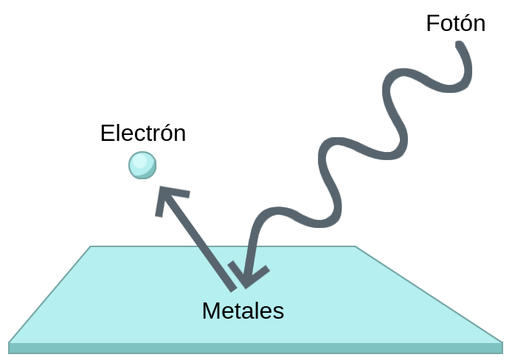
\includegraphics[width=6cm]{../imagenes/LGH_PhotoelectricEffect.es_ES.x512.png}};
    \node at (17cm, -7cm) {\scalebox{5}{\textbf{U}}};
    \node at (17cm, -9cm) {\scalebox{5}{\textbf{T}}};
    \node at (17cm, -11cm) {\scalebox{5}{\textbf{N}}};
    \node at (17cm, -14cm) {\scalebox{5}{\textbf{F}}};
    \node at (17cm, -16cm) {\scalebox{5}{\textbf{R}}};
    \node at (17cm, -18cm) {\scalebox{5}{\textbf{C}}};
    \node at (7.25cm, -12cm) {\scalebox{2}{\textbf{EFECTO FOTOELÉCTRICO}}};

    \node at (7.5cm, -22cm) {\begin{minipage}[c]{12cm}
      \begin{itemize}
          \raggedright
          \vspace{1.5cm}
                \item \fontsize{12}{12}\selectfont \textbf{Autores:} \vspace {1mm} \fontsize{11}{12}\selectfont \\
                    \begin{itemize}
                        \item \hspace{2mm} Valentino Rao - Leg. 402308 \\
                        \item \hspace{2mm} Ignacio Ismael Perea - Leg. 406265 \\
                        \item \hspace{2mm} Manuel Leon Parfait - Leg. 406599 \\
                        \item \hspace{2mm} Gonzalo Filsinger - Leg. 400460 \\
                        \item \hspace{2mm} Agustín Coronel - Leg. 402010 \\
                        \item \hspace{2mm} Marcos Raúl Gatica - Leg. 402006 \\
                    \end{itemize}

                \item \fontsize{12}{12}\selectfont \textbf{Curso:} 2R1. \\
                \item \fontsize{12}{12}\selectfont \textbf{Asignatura:} Física electrónica. \\
                \item \fontsize{12}{12}\selectfont \textbf{Institución:} Universidad Tecnológica Nacional - Facultad Regional de Córdoba \\
      \end{itemize}
    \end{minipage}};

\end{tikzpicture}

\renewcommand{\normalsize}{\fontsize{12}{18}\selectfont}
\newgeometry{margin=1cm}
\fancyhf{}
\renewcommand{\headrulewidth}{0pt} 
\renewcommand{\footrulewidth}{0pt}
\fancyfoot[R]{[Rao V. - Perea I. - Parfait M. - Filsinger G. - Coronel A. - Gatica M.] [\textbf{pág. \thepage]}}
\setlength{\footskip}{0pt} % explain this line: 

\newpage
\thispagestyle{empty}
\text{}

\titleformat{\section} {\fontsize{12}{12}\bfseries}{\thesection.}{0.5em}{\underline}

\newpage

\thispagestyle{empty}
\setcounter{page}{0}
\tableofcontents
\newpage
\thispagestyle{fancy}


\twocolumn
  \flushbottom
    \section{INTRODUCCIÓN}
      \subsection{Electroscopio de Wulf}
        \indent El electroscopio de Wulf es un instrumento que se utiliza para medir el efecto fotoeléctrico. Este fenómeno se produce cuando un material emite electrones al ser iluminado por una fuente de luz. El electroscopio de Wulf consta de una placa metálica de zinc que se encuentra conectada a un electroscopio. Cuando la placa es iluminada por una fuente de luz, los electrones emitidos por el zinc se acumulan en el electroscopio, produciendo una carga eléctrica. Adentro de electroscopio hay una chapa soldada a un hilo de cobre, cuando el electroscopio se carga y el cable toca tierra la chapa metalica vibra.\\

        \begin{figure}[h]
          \centering
          \includegraphics[width=4.5cm]{../imagenes/electroscopio.jpg}
          \caption{\small Electroscopio de Wulf}
        \end{figure}

    \section{PRIMERA EXPERIENCIA}
      \subsection{Energía como función de la intensidad de la luz}
        \indent En la experiencia realizada medimos como la energía potencial de la luz es función de la intensidad de la luz. Para ello, se utilizó una fuente luminosa de vapor de mercurio haciendo que impacte en un foto diodo, el cual tenia dos filtro, uno de color amarillo/verde y uno el cual dejaba pasar solo una cierta cantidad de luz. A continuacion las imagenes de los objetivos utilizados.

        \begin{figure}[h]
          \centering
          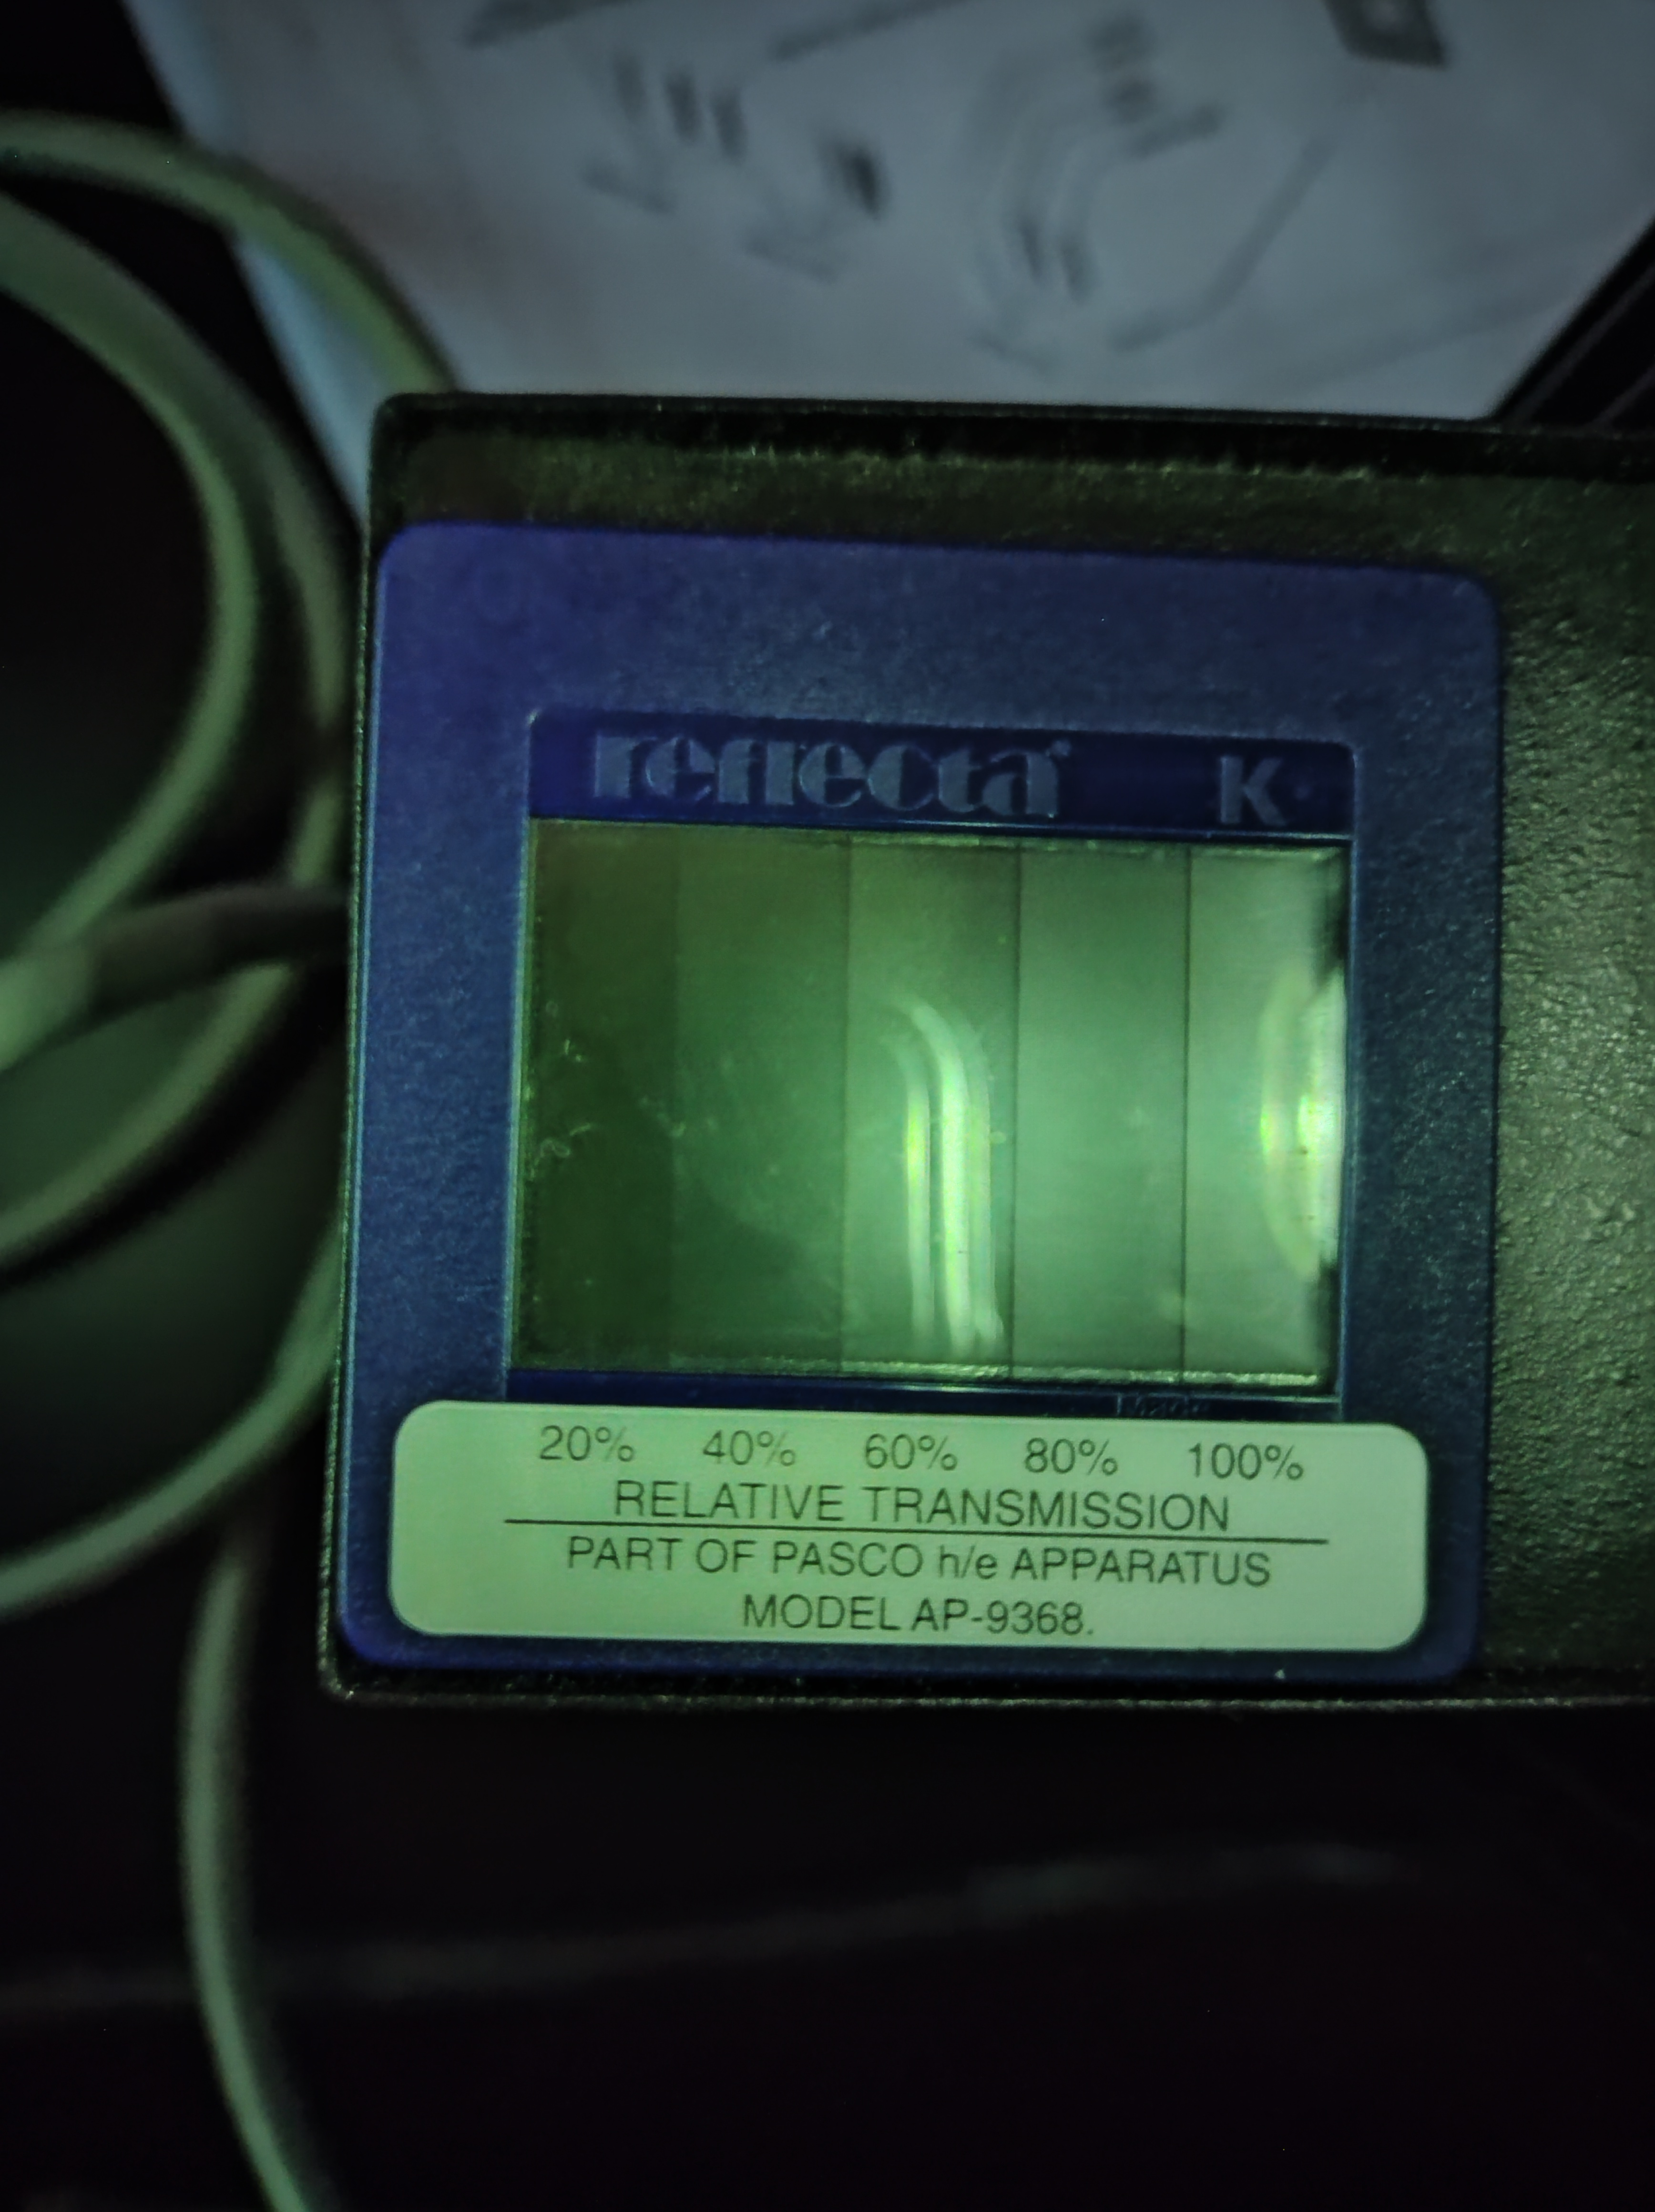
\includegraphics[trim={0 30cm 0 30cm},clip,width=4.5cm]{../imagenes/filtro1.jpg}
          \caption{\small Filtro 1}
        \end{figure}

        \begin{figure}[h]       
          \centering
            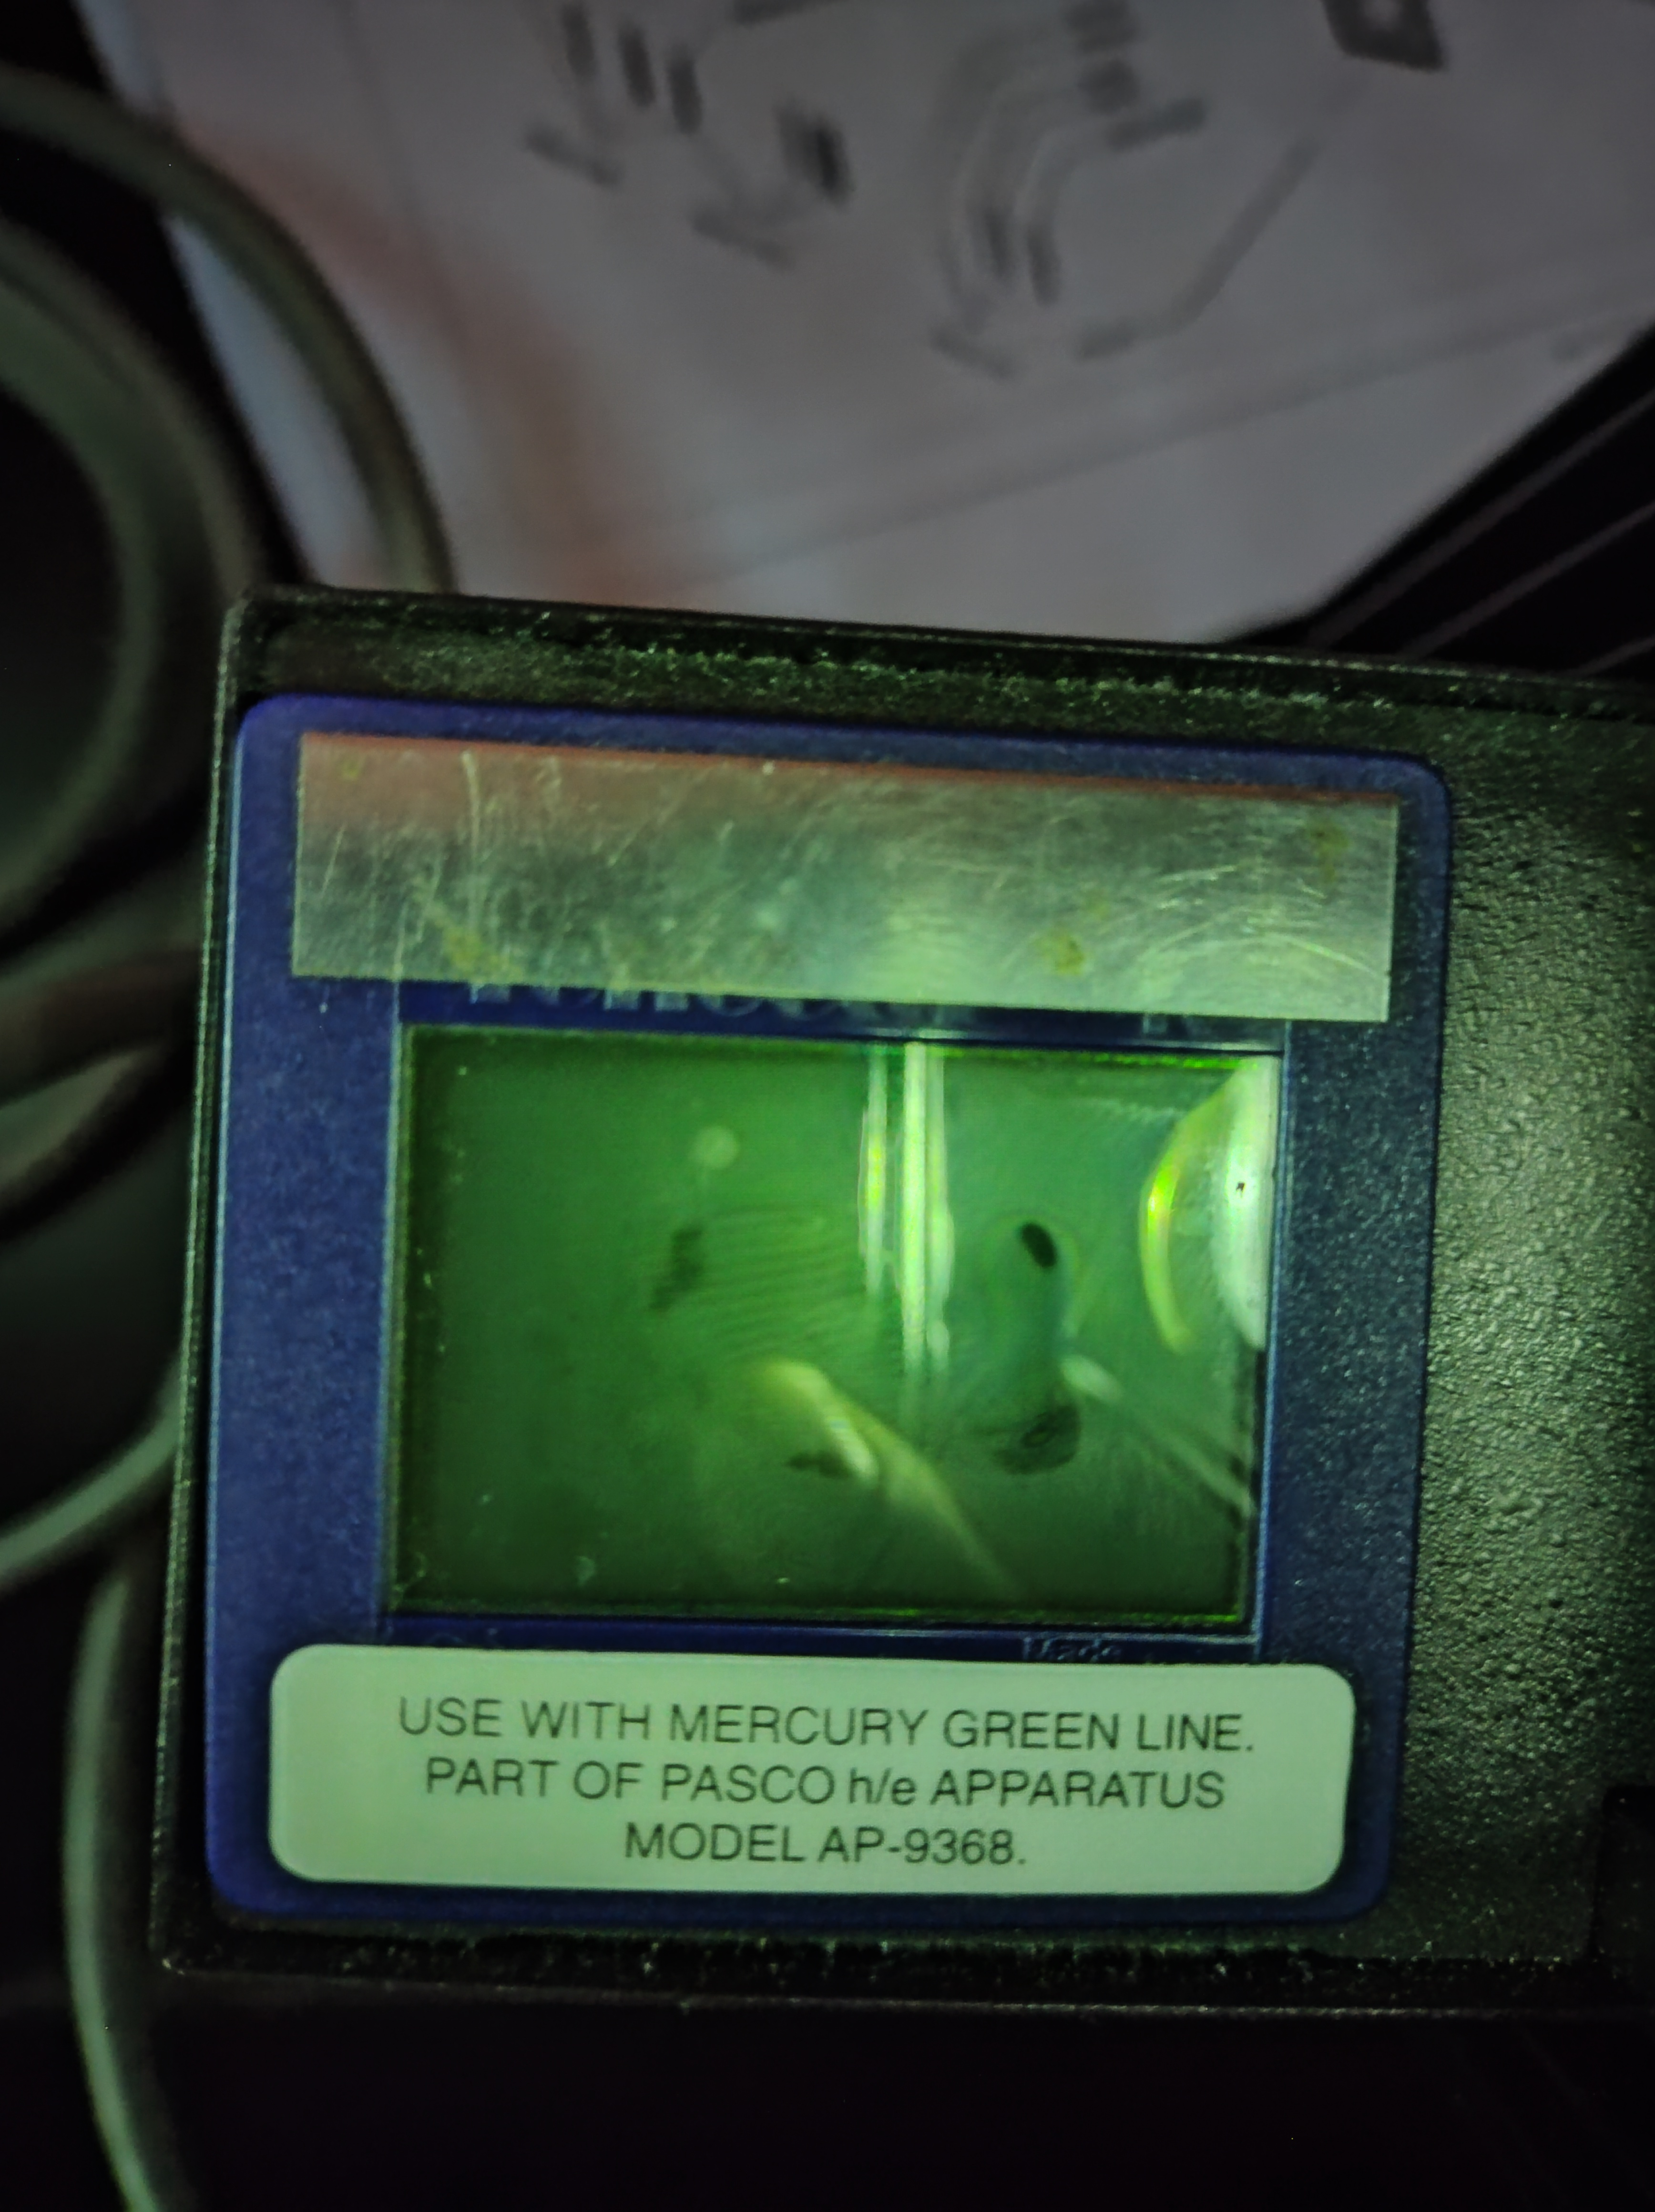
\includegraphics[trim={0 30cm 0 30cm},clip,width=4.5cm]{../imagenes/filtro2.jpg}
            \caption{\small Filtro 2}
        \end{figure}
          
        \begin{figure}[h]
                \centering
                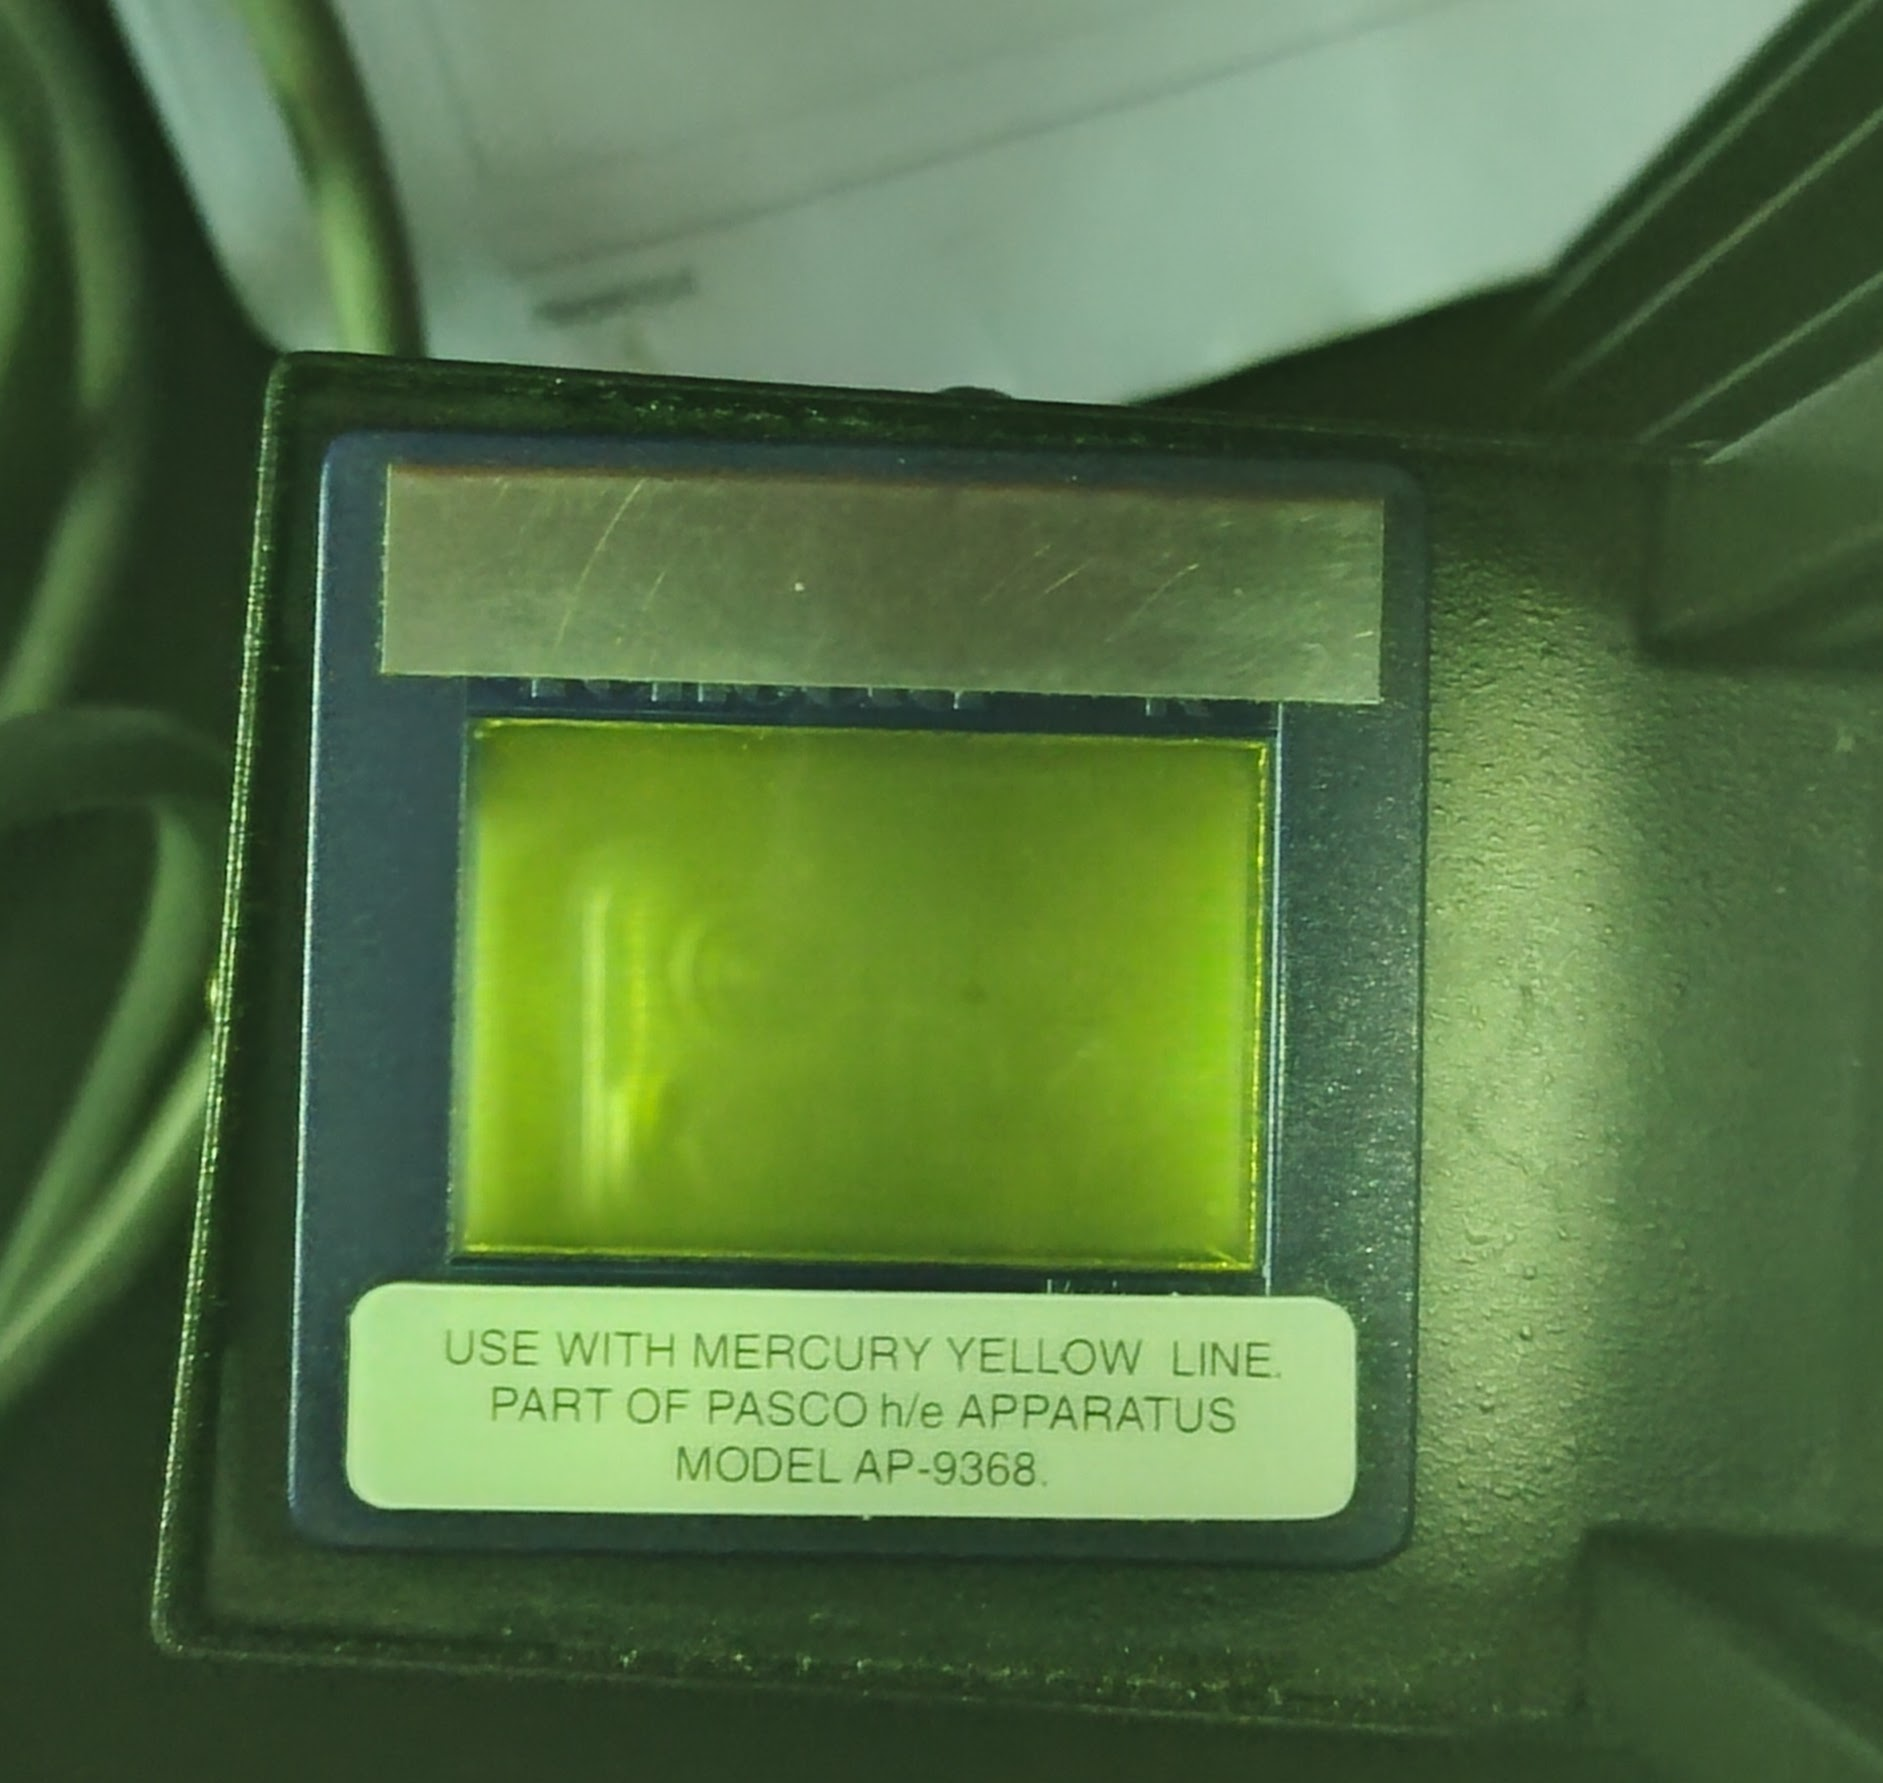
\includegraphics[width=4.5cm]{../imagenes/filtro3.jpg}
                \caption{\small Filtro 3}
        \end{figure}
        \vspace{5mm}
        
        \indent Luego de realizar la experiencia, se obtuvieron los siguientes resultados:

        \begin{minipage}[c]{7.5cm}
          \vspace{2mm}
          \centering
          \textit{Amarillo} 
          \vspace{1mm}
        \end{minipage}
        
      \begin{center}
        \begin{tabular}{ c c c c c }
            \toprule
            Intensidad ($\%$) & Energía $V_{0}$ (mV) & Tiempo (s) \\
              \midrule
              100 & 234,3 & 33\\
              80 & 221 & 55\\
              60 & 212 & 40\\
              40 & 184 & 63\\
              20 & 150 & 33\\
            \bottomrule
          \end{tabular}
        \end{center}

          \begin{minipage}[c]{7.5cm}
            \vspace{5mm}
            \centering
            \textit{Verde} 
            \vspace{1mm}
          \end{minipage}

        \begin{center}
          \begin{tabular}{ c c c c c }
            \toprule
            Intensidad ($\%$) & Energía $V_{0}$ (mV) & Tiempo (s) \\
              \midrule
              100 & 302,5 &    52   \\
              80 & 300    &    52   \\
              60 & 278    &    63   \\
              40 & 248    &    61   \\
              20 & 198,5  &    58   \\
            \bottomrule
          \end{tabular}
        \end{center}

        \indent A continuación se muestra el gráfico de los resultados obtenidos:

        \begin{figure}[h]
          \centering
          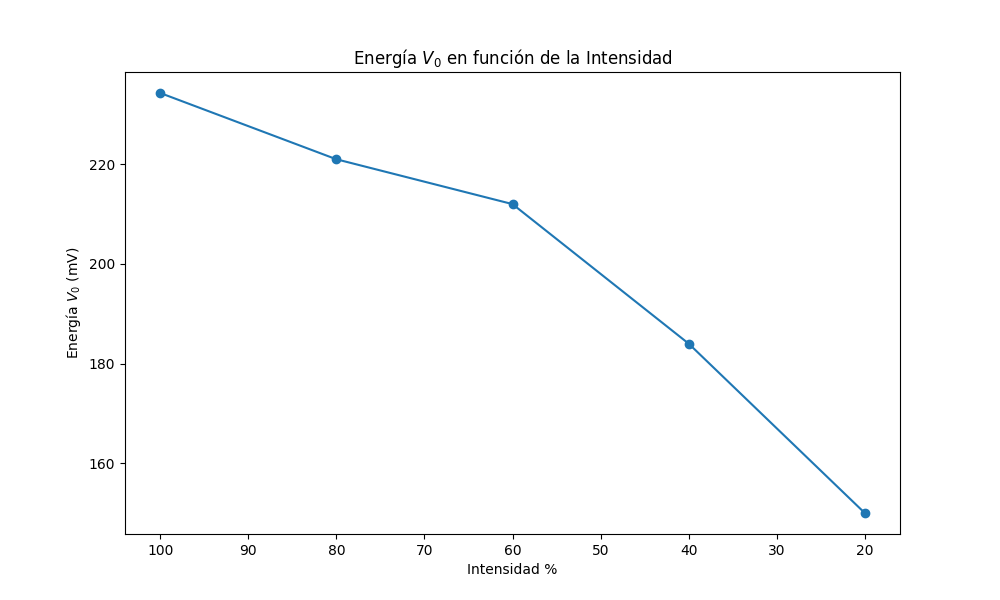
\includegraphics[width=6.7cm]{../imagenes/amarillo_energia_intensidad.png}
          \caption{\small Energía como función de la intensidad de la luz}
        \end{figure}

        \begin{figure}[h]
          \centering
          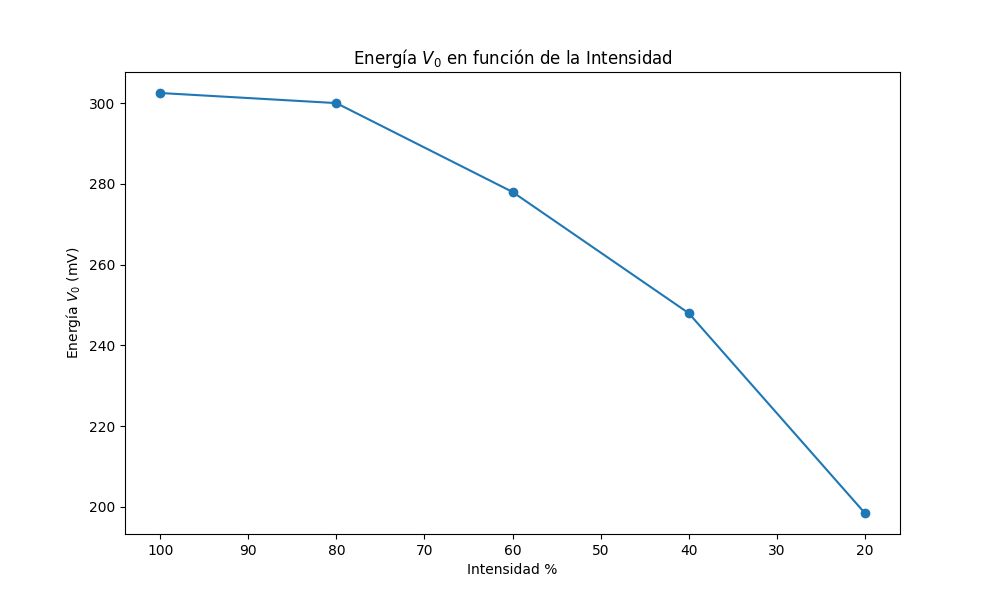
\includegraphics[width=6.7cm]{../imagenes/verde_energia_intensidad.png}
          \caption{\small Energía como función de la intensidad de la luz}
        \end{figure}
        
        \newpage
        \noindent
        \thispagestyle{fancy}
        
        
        \subsection{Conclusiones:}
        \indent Como se puede observar en los gráficos, la energía potencial de corte $V_{0}$ es función de la intensidad de la luz. A medida que la intensidad de la luz disminuye, la energía potencial de corte $V_{0}$ también disminuye.\\
        \indent En el caso del color amarillo, la energía potencial de corte $V_{0}$ disminuye de 234,3 mV a 150 mV a medida que la intensidad de la luz disminuye de 100$\%$ a 20$\%$. En el caso del color verde, la energía potencial de corte $V_{0}$ disminuye de 302,5 mV a 198,5 mV a medida que la intensidad de la luz disminuye de 100$\%$ a 20$\%$.\\
        \indent En conclusión, la energía potencial de corte $V_{0}$ es función de la intensidad de la luz. A medida que la intensidad de la luz disminuye, la energía potencial de corte $V_{0}$ también disminuye.

    \section{SEGUNDA EXPERIENCIA}
      \subsection{Constante de Planck}
      \indent En esta segunda experiencia medimos la energía potencial de corte $V_{0}$ del 1er y 2do orden, con un electroscopio PASCO. Para ello, se utilizó una fuente luminosa de vapor de mercurio, la cual impactaba en un fotodiodo. Con este dispositivo se midió la energía potencial de corte $V_{0}$ de los colores amarillo, verde, azul, violeta y ultravioleta. Esta es una representación del objetivo utilizado.

      \begin{figure}[h]
        \centering
        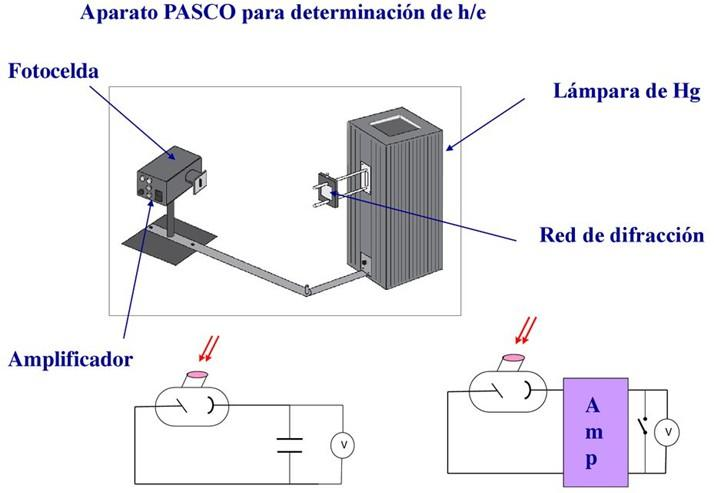
\includegraphics[width=6cm]{../imagenes/dispositivo_2daexperiencia.jpg}
        \caption{\small Fotodiodo}
      \end{figure}

      \indent Luego de realizar la experiencia, se obtuvieron los siguientes resultados:

      \begin{minipage}[c]{7.5cm}
        \vspace{5mm}
        \centering
        \textit{1er orden} 
        \vspace{2mm}
      \end{minipage}

      \begin{tabular}{ c c c }
        \toprule
        Color & Frecuencia ($\times 10^{14}$ Hz) & Energía $V_{0}$ (mV)\\
          \midrule
          Amarillo      & 5,186 & 435   \\
          Verde         & 5,489 & 450   \\
          Azul          & 6,878 & 1130  \\
          Violeta       & 7,408 & 1230  \\
          Ultravioleta  & 8,202 & 1000  \\
        \bottomrule
      \end{tabular}

      \begin{minipage}[c]{7.5cm}
        \vspace{5mm}
        \centering
        \textit{2do orden} 
        \vspace{2mm}
      \end{minipage}

      \begin{tabular}{ c c c }
        \toprule
        Color & Frecuencia ($\times 10^{14}$ Hz) & Energía $V_{0}$ (mV) \\
          \midrule
          Amarillo      & 8,184 & 234,3 \\
          Verde         & 7,400 & 302,5 \\
          Azul          & 6,849 & 1000  \\
          Violeta       & 5,890 & 1800  \\
          Ultravioleta  & 5,190 & 800   \\
        \bottomrule
      \end{tabular}

\newpage
\noindent
\thispagestyle{fancy}

      \indent El gráfico de los resultados obtenidos es el siguiente:

      \begin{figure}[h]
        \centering
        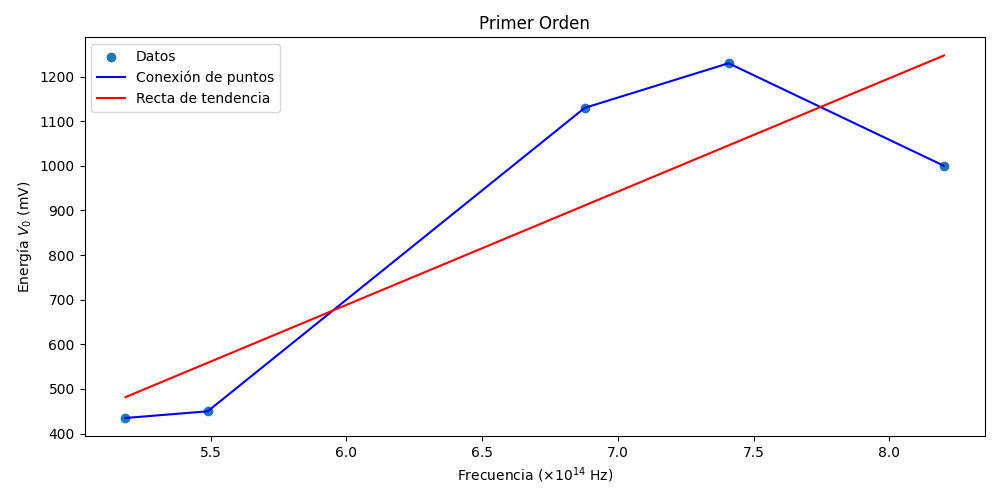
\includegraphics[width=6.7cm]{../imagenes/1er_orden.png}
        \caption{\small 1er orden del espectro}
      \end{figure} 

      \begin{figure}[ht]
        \centering
        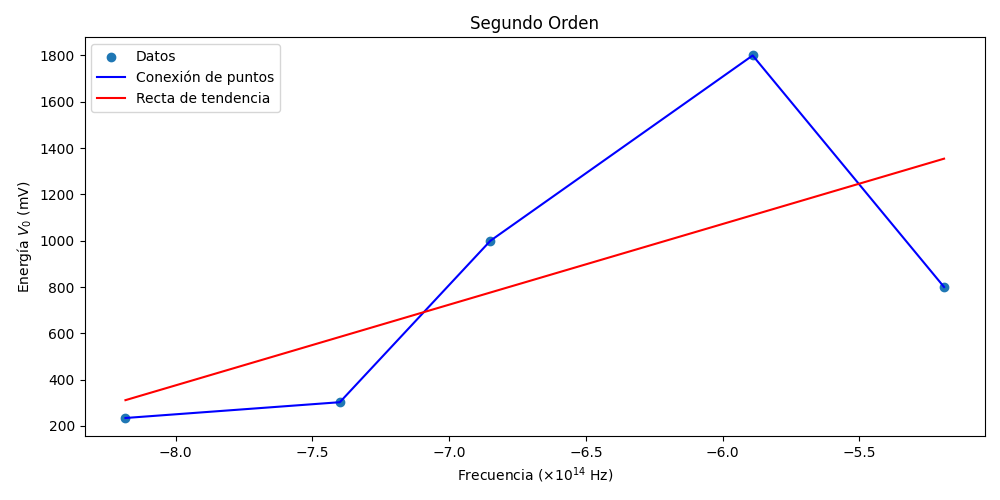
\includegraphics[width=6.5cm]{../imagenes/2do_orden.png}
        \caption{\small 2do orden del espectro}
      \end{figure}
      \vspace{5mm}

      \indent El promedio de las energías potenciales de corte $V_{0}$ y frecuencias para cada color es:\\
      \begin{center}
        \textit{Promedio 1er orden y 2do orden}  
      \end{center}

      \begin{center}
        \begin{tabular}{ c c c }
          \toprule
          Color & Frecuencia ($\times 10^{14}$ Hz) & Energía $V_{0}$ (mV) \\
            \midrule
            Amarillo      & 6,636 & 964   \\
            Verde         & 6,503 & 827,4 \\
            Azul          & 6,864 & 1065  \\
            Violeta       & 6,649 & 1515  \\
            Ultravioleta  & 6,696 & 900   \\
          \bottomrule
        \end{tabular}
      \end{center}
      \vspace{5mm}

      \begin{figure}[h]
        \centering
        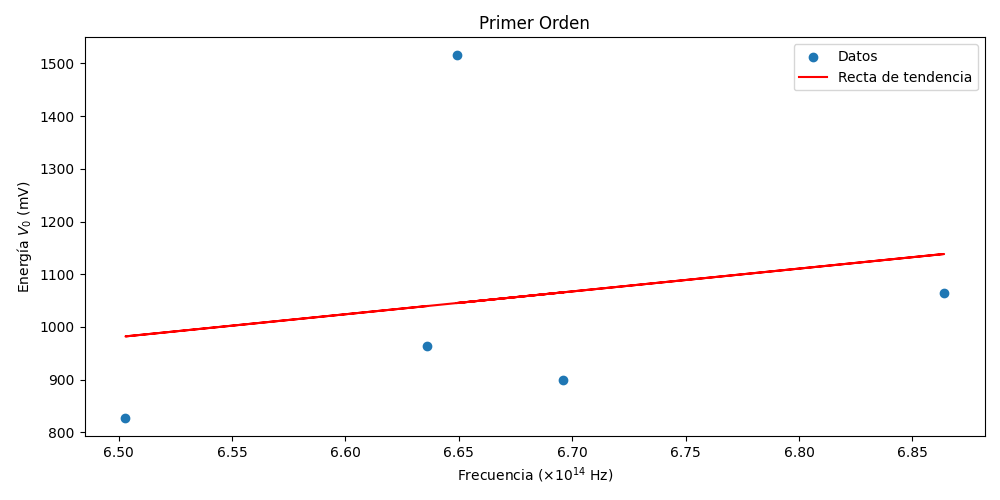
\includegraphics[width=6.5cm]{../imagenes/promedio1ery2do_orden.png}
        \caption{\small Promedio de 1er y 2do orden del espectro}
      \end{figure}
      \vspace{5mm}

      \indent La pendiente de la recta tiene un valor de $3,8 \times 10^{-15}$ Hz.
      \vspace{5mm}

      \begin{minipage}[c]{7.5cm}
        \vspace{5mm}
        \centering
        \textit{Promedio 1er orden} 
        \vspace{2mm}
      \end{minipage}

      \begin{center}
        \begin{tabular}{ c c }
          \toprule
           Frecuencia ($\times 10^{14}$ Hz) & Energía $V_{0}$ (mV) \\
            \midrule
             6,636 & 964 \\
          \bottomrule
        \end{tabular}
      \end{center}

      \newpage
      \noindent
      \thispagestyle{fancy}

      \begin{minipage}[c]{7.5cm}
        \vspace{5mm}
        \centering
        \textit{Promedio 2do orden} 
        \vspace{2mm}
      \end{minipage}
      
      \begin{center}
        \begin{tabular}{ c c }
          \toprule
           Frecuencia ($\times 10^{14}$ Hz) & Energía $V_{0}$ (mV) \\
            \midrule
            6,503 & 827,4 \\
          \bottomrule
        \end{tabular}
      \end{center}

      \vspace{5mm}
      
      \begin{minipage}[c]{7.5cm}
        \vspace{5mm}
        \centering
        \textit{Promedio de todas las frecuencias y energías potenciales de corte} 
        \vspace{2mm}
      \end{minipage}
     
      \begin{center}
        \begin{tabular}{ c c }
          \toprule
           Frecuencia ($\times 10^{14}$ Hz) & Energía $V_{0}$ (mV) \\
            \midrule
             6,569 & 895,7 \\
          \bottomrule
        \end{tabular}
      \end{center}
      \vspace{5mm}

      \indent A partir de los resultados obtenidos, según la ecuación de Einstein:
      
      \begin{equation}
        W = h \cdot f - eV_{0}
      \end{equation}
      \indent Podemos despejar $V_{0}$, quedando de la siguiente manera:
      \begin{equation}
        V_{0} = \frac{h}{e} \cdot f - \frac{W}{e}
      \end{equation}

      \vspace{5mm}

      \indent Segun la ecuación (2) $V_{0}$ es función de $f$, obteniendo una recta. Si tomamos una ecuación lineal representada por la fórmula $y = mx + b$, donde $y$ es $V_{0}$, $x$ es $f$, $b$ es la ordenada al origen, en este caso, $W$ y  la pendiente de la recta $m$ es $\frac{h}{e}$.\\
      \indent Donde $W$ es la energía cinética de los electrones, $h$ es la constante de Planck, $f$ es la frecuencia de la luz y $V_{0}$ es la energía potencial de corte. Segun la ecuación(1), se puede calcular la energía cinética de los electrones, para 1er y 2do orden del espectro, sacando el promedio de los valores obtenidos.\\
      \indent En el caso del 1er orden del espectro, el promedio de las frecuencias es de $6,636 \times 10^{14}$ Hz y el promedio de las energías potenciales de corte $V_{0}$ es de 964 mV. Sustituyendo estos valores en la ecuación (1), se obtiene que la energia cinetíca de los electrones es $W = 3,2 \times 10^{-19}$J.En el caso del 2do orden del espectro, el promedio de las frecuencias es de $6,503 \times 10^{14}$ Hz y el promedio de las energías potenciales de corte $V_{0}$ es de 827,4 mV. Sustituyendo estos valores en la ecuación (1), se obtiene que la energia cinetíca de los electrones es $W = 3,2 \times 10^{-19}$J.\\
      \indent A partir de los resultados obtenidos, se puede calcular el promedio de $W$, el cual es de $3,2 \times 10^{-19}$J. El promedio de las frecuencias $f$ es de $6,569 \times 10^{14}$ Hz y el promedio de las energías potenciales de corte $V_{0}$ es de 895,7 mV. Sustituyendo estos valores en la ecuación (1), se obtiene que la constante de Planck $h$ es de $6,1 \times 10^{-34}$J/s. Este mismo resultado tambien se puede observa en el gráfico (10), ya que la pendiente de la recta es $\frac{h}{e}$, donde $e$ es la carga del electrón, la cual es de $1,6 \times 10^{-19}$C. En nuestro grafico la pendiente tuvo un valor de $3,8 \times 10^{-15}$Hz, si multiplicamos este valor por la carga del electrón, obtenemos el valor de la constante de Planck $h$, el cual es de $6,1 \times 10^{-34}$J/s.\\
      
    \section{CONCLUSIONES}
    \indent En la segunda experiencia, se pudo observar que la energía potencial de corte $V_{0}$ es función de la frecuencia de la luz. A medida que la frecuencia de la luz aumenta, la energía potencial de corte $V_{0}$ también aumenta. 
    
\newpage
\noindent
\thispagestyle{fancy}
    \indent A partir de los resultados obtenidos, se pudo calcular la constante de Planck $h$, la cual nos dió un resultado de:
    

    \begin{equation}
      h = 6,1 \times 10^{-34} J/s
    \end{equation}
    

    \indent Esto concuerda con el valor de la constante de Planck $h$, la cual es de $6,63 \times 10^{-34} J/s$, nuestro resultado posee un error de $8,6\%$. Este error puede deberse a la precisión de los instrumentos utilizados, a la calibración de los mismos y a la medición de los datos.\\
    \indent Mientras que para la energía cinetíca de los electrones ($W$), se midió un valor de:
    

    \begin{equation}
      W = 3,2 \times 10^{-19} J
    \end{equation}

    \indent El cual es el mismo para el 1er y 2do orden del espectro y posee un error con respecto al valor teórico de $3,6 \times 10^{-19}$J del $11,1\%$.\\
    \indent En conclusión, la energía potencial de corte $V_{0}$ es función de la frecuencia de la luz. A medida que la frecuencia de la luz aumenta, la energía potencial de corte $V_{0}$ también aumenta. También podemos deducir que el potencial de corte $V_{0}$ es función de la intensidad de la luz, ya que a medida que la intensidad de la luz disminuye, la energía potencial de corte $V_{0}$ también disminuye.

\end{document}
